\documentclass{article}
\usepackage{amsmath, amssymb, amsthm, amsfonts, bm}
\theoremstyle{remark}
\newtheorem*{theorem}{Theorem}
\newtheorem*{remark}{Remark}
\newtheorem*{definition}{Definition}
\newtheorem*{hypothesis}{Hypothesis}
\newtheorem*{corollary}{Corollary}
\theoremstyle{remark}

\usepackage{physics}
\usepackage[a4paper, total={6in,10in}]{geometry}
\usepackage[dvipsnames]{xcolor}
\usepackage{hyperref}
    \hypersetup{colorlinks=true, linkcolor=ForestGreen}
\usepackage{graphicx}
    \graphicspath{{./img/}}
\usepackage{tikz}
\usepackage{ragged2e}
\usepackage{array}   % for \newcolumntype macro
\newcolumntype{L}{>{$}c<{$}} % math-mode version of "l" column type

\usepackage{soul}
\everymath{\displaystyle}

\usepackage{empheq}
\usepackage{framed}
\usepackage{mathtools}

\newcommand{\where}[1]{\begin{flushright}where #1.\end{flushright}}
\newcommand{\wher}[1]{\begin{flushright}#1.\end{flushright}}
\newcommand{\mylabel}[2]{\hyperref[#1]{#2}\label{back:#1}}
\newcommand{\myref}[1]{\hyperref[back:#1]{$\bigstar$}\label{#1}}
\newcommand{\e}{\hat{\vb{e}}}  % unit vector
\newcommand{\realp}[1]{\mathfrak{R}(#1)}
\begin{document}

\title{Quantum Notes}
\maketitle

\subsubsection*{Section 1}
\begin{enumerate}
    \item $h=6.63\times 10^{-34} \mathrm{Js}$, $\hbar=\frac{h}{2\pi}$
    \item Fine structure constant $\alpha=\frac{1}{4\pi\epsilon_0}\frac{e^2}{\hbar c}\approx\frac{1}{137}$
    \item Photoelectric effect $E=h\nu=\hbar\omega$, $eV_0=h\nu-W$
    \item de Broglie wavelength $p=h/\lambda, \vb{p}=\hbar\vb{k}$
    \item Angular momentum of electron $L=n\hbar$, $n$ is the principal quantum number
    \item $\omega=\frac{\hbar k^2}{2m}$
    \item $\Phi(\vb{r},t)=Ae^{i(\vb{k}\cdot\vb{r}-\omega t)} = Ae^{\frac{i}{h}(\vb{p}\cdot\vb{r}-Et)}$ (not really meaningful unless $|\Phi(\vb{r},t)|\rightarrow0$)
    \item A localized wavefunction is $\Phi(x,t)=\frac{1}{\sqrt{2\pi}}\int_{-\infty}^{+\infty} g(k)e^{i(kx-\omega t)}\dd k$, $g(k,t)=\frac{1}{\sqrt{2\pi}}\int_{-\infty}^{+\infty}\Phi(x,t)e^{-i(kx-\omega t)}\dd x$, $\int_\infty^\infty |g(k,t)|^2\dd k=\int_\infty^\infty |\Phi(x,t)|^2\dd x$, $g(k)$ is the momentum wavefunction.
    \item $\langle x\rangle=\int_{-\infty}^{+\infty}x P(x)d x=\int_{-\infty}^{+\infty}x|\Psi(x)|^{2}d x$
    \item $\langle x^{2}\rangle=\int_{-\infty}^{+\infty}x^{2}P(x)d x=\int_{-\infty}^{+\infty}x^{2}|\Psi(x)|^{2}d x$
    \item $\Delta x=\sqrt{\langle x^{2}\rangle-\langle x\rangle^{2}}$
    \item Wavepacket $g(k)=\left(\frac{a^2}{\pi}\right)^{1/4}e^{-a^2(k-k_0)^2/2}$, \begin{itemize}
        \item $\Psi(x,0)=\left(\frac{1}{\pi a^2}\right)^{1/4}e^{ik_0x}e^{-x^2/2a}$
        \item $\Psi(x,t)=e^{i k_{0}(x-v_{p}t)}f(x-v_{g}t)$
        \item $\langle x\rangle=\left(\frac{1}{\pi a^{2}}\right)^{1/2}\int_{-\infty}^{+\infty}x e^{-(x^{2}/a^{2})}d x=0$
        \item $\langle x^{2}\rangle=\left(\frac{1}{\pi a^{2}}\right)^{1/2}\int_{-\infty}^{+\infty}x^{2}e^{-(x^{2}/a^{2})}d x=\frac{a^2}{2}$
        \item $\left\langle k\right\rangle=\left(\frac{a^{2}}{\pi}\right)^{1/2}\int_{-\infty}^{+\infty}k e^{-a^{2}(k-k_{0})^{2}}d k=k_{0}$
        \item $\left\langle k^{2}\right\rangle=\left(\frac{a^{2}}{\pi}\right)^{1/2}\int_{-\infty}^{+\infty}k^{2}e^{-a^{2}(k-k_{0})^{2}}d k=\frac{1}{2a^{2}}+k_{0}^{2}$
        \item $\Delta x={\frac{a}{\sqrt{2}}}\;\;\mathrm{and}\;\;\Delta p={\frac{\hbar}{a\sqrt{2}}}$
        \item $\Delta x\Delta p={\frac{\hbar}{2}}$
    \end{itemize}
    \item $\Delta x\Delta p_y=0$ is possible, spatially orthogonal quantities can be measured simultaneously to any precision
    \item Time evolution of a gaussian $\omega=\frac{\hbar k^2}{2m}$,$g(k)=\left(\frac{a^{2}}{\pi}\right)^{1/4}e^{-a^{2}(k-k_{0})^{2}/2}$, 
    
    \begin{align*}
        \Psi(x,t)&={\frac{1}{\sqrt{2\pi}}}\int_{-\infty}^{+\infty}g(k)e^{i\left[k x-\omega(k)t\right]}d k \\
                 &=\frac{1}{\sqrt{2\pi}}\left(\frac{a^{2}}{\pi}\right)^{1/4}\int_{-\infty}^{+\infty}e^{-a^{2}\delta k^{2}/2}e^{i\left[(k_{0}+\delta k)x-\left(\omega_{0}+\alpha\delta k+\beta(\delta k)^{2}\right)t\right]}d(\delta k)\\
                 &\left(\alpha=\frac{\hbar k_0}{m},\ \beta=\frac{\hbar}{2m}\right)\\
        |\Psi(x,t)|^2 &= \left(\frac{a^{2}}{4\pi}\right)^{1/2}\frac{1}{(a^{4}/4+h^{2}t^{2}/4m^{2})^{1/2}}\exp\left\{\frac{-(x-\hbar k_{0}t/m)^{2}}{(a^{2}+h^{2}t^{2}/m^{2}a^{2})}\right\}\\
        \langle x\rangle &= \hbar k_0t/m = v_g t\\
        (\Delta x)^2 &= a^2/2(1+\hbar^2t^2/a^4m^2)
    \end{align*}

    \item $\Phi(p,t)={\frac{1}{\sqrt{\hbar}}}\,g\left({\frac{p}{\hbar}},t\right)$, 
    
        $\Psi(x,t)=\frac{1}{\sqrt{2\pi\hbar}}\int_{-\infty}^{+\infty}\Phi\bigl(p,t\bigr)e^{i p x/\hbar}d p$, 
    
        $\Phi(p,t)={\frac{1}{\sqrt{2\pi\hbar}}}\int_{-\infty}^{+\infty}\Psi(x,t)e^{-i p x/\hbar}d x$

    Gaussian $\Phi(p,0)=\left({\frac{a^{2}}{\pi\hbar^{2}}}\right)^{1/4}\exp^{-a^{2}(p-p_{0})^{2}/2\hbar^{2}}$

    \item Total energy operator/Hamiltonian $\hat{E} \equiv i\hbar\pdv{t}$
    
    Total momentum operator $\hat{p}\equiv -i\hbar\pdv{x}$, $\vb{\hat{p}}=-i\hbar\grad$

    Kinetic energy operator $\frac{\hat{p}^2}{2m}\equiv -\frac{h^2}{2m}\pdv[2]{x} = -\frac{\hbar^2}{2m}\laplacian$

    The eigenvalues of an operator are the possible values that might be returned by an experiment.


    \item $\hat{E}=\frac{\hat{p}^2}{2m}+\hat{V}(x,t)=\hat{E}$
    
        $\boxed{i\hbar\pdv{\Psi(x,t)}{t}}=-\frac{\hbar^2}{2m}\pdv[2]{\Psi(x,t)}{x}+V(x,t)\Psi(x,t)$

        $i\hbar\pdv{\Psi(\vb{r},t)}{t}=-\frac{\hbar^2}{2m}\laplacian{\Psi(\vb{r},t)}+V(\vb{r},t)\Psi(\vb{r},t)$

        Let $\Psi(x,t)=\Psi(x)T(t) = \Psi(x)e^{-iEt/\hbar}$, time-independent Schr\"odinger is $-\frac{h^2}{2m}\laplacian{\Psi(\bm{r})}+V(\bm{r})\Psi(\bm{r})=E\Psi(\bm{r})$

    \item If $V(\vb{r},t)=V(\vb{r})$, $\Psi(\vb{r},t)=\psi(\vb{r})T(t)$
    
        $-\frac{\hbar^{2}}{2m}\nabla^{2}\psi({\bf r})+V({\bf r})\psi({\bf r})=E\psi({\bf r})$

        $-\frac{\hbar^{2}}{2m}\nabla^{2}\psi({\bf r})+V({\bf r})\psi({\bf r})=E\psi({\bf r})$

    \item $i\hbar\pdv{t}\int_{\mathcal{V}}P(\mathbf{r},t)d V=i\hbar\pdv{t}\int_{\mathcal{V}}\Psi^{\ast}(\mathbf{r},t)\Psi(\mathbf{r},t)d V$
    
        $\boxed{{\frac{\partial}{\partial t}}\int_{\mathcal{V}}P(\mathbf{r},t)d V=-\oint_{S}\mathbf{J}(\mathbf{r},t)\cdot d\mathbf{s}}$
        
        $\pdv{P}{t}+\div\vb{J} = 0$

        \begin{align*}\mathbf{J}(\mathbf{r},t)&=\frac{\hbar}{\dot{\imath}2m}\bigl[\Psi^{*}\bigl(\mathbf{r},t\bigr)\nabla\Psi(\mathbf{r},t)-\Psi(\mathbf{r},t)\nabla\Psi^{*}\bigl(\mathbf{r},t\bigr)\bigr]  \\
            &= \Re[\Psi^{\star}(\vb{r}, t)\frac{\hbar}{im}\grad\Psi(\vb{r},t)] \\
            &= \Re[\Psi^{\star}(\vb{r}, t)\frac{\hat{\vb{p}}}{m}\grad\Psi(\vb{r},t)]\end{align*}

    For $\Psi(x,t)=Ae^{i(kx-\omega t)}$, $\boxed{J=v|A|^2=\frac{\hbar k}{m}|A|^2}$
    \item SHO $V(x)=\frac{1}{2}m\omega^2 x^2$, $q=x\sqrt{\frac{m\omega}{\hbar}}$, $\epsilon=\frac{2E}{\hbar\omega}$, $\chi(q)=\psi(q\sqrt{\frac{\hbar}{m\omega}})=H(q)e^{-q^2/2}$\begin{align*}
        &\pdv[2]{H(q)}{q}-2q\pdv{H}{q}+(\epsilon-1)H(q) = 0\\
        &H_n(q)=(-1)^n e^{q^2}\dv[n]{q}\left(e^{-q^2}\right)\\
        &E_n=\left(n+\frac{1}{2}\right)\hbar\omega\\
        &\psi_n=A_n H_n\left[x\sqrt{\frac{m\omega}{\hbar}}\right]e^{-\frac{m\omega}{2\hbar}x^2}\\
        &A_n = \left[\sqrt{\frac{\hbar}{m\omega}}\sqrt{\pi}2^n n!\right]^{-1/2}
    \end{align*}
    \item Parity operator $\hat{P}\psi(\vb{r}) = \psi(-\vb{r})$
    \item For bounded systems, $psi(x)=\sum_{n=1}^{\infty}a_n\psi_n(x)$, $\ket{a}=\sum_n a_n\ket{a}_n$
    \item Completeness relation (bounded system) $\sum_{n=1}^{\infty}\psi_n(x)\psi_n^*(y)=\delta(x-y)$, $\sum_{n=1}^{N}\vb{a}_n\vb{a}_n^\dagger=I$,\allowbreak $\sum_n\ket{a}\bra{a}=\hat{I}$
    \item For unbounded systems, $\psi(x)=\int\phi(k)\chi(x,k)\dd k$, $\int_{-\infty}^\infty\chi^*(k,x_1)\chi(k,x_2)\dd k=\delta(x_2-x_1)$
    \item Commutator $\left[\hat{A},\hat{B}\right]\equiv \hat{A}\hat{B}-\hat{B}\hat{A}$
    \item $A_{nm}\equiv\bra{u_n}\hat{A}\ket{u_m}$, $\hat{A}\equiv\sum_{n,m}A_{nm}\ket{u_n}\bra{u_m}$ (opeartor as linear combination of outer products)
    \item Operators like $\hat{P}=\ket{\psi}\bra{\psi}$ is a projection operator
    \item The adjoint of an operator is $\hat{A}^\dagger$\begin{itemize}
        \item $\bra{u_m}\hat{A}\ket{u_n}=\bra{u_n}\hat{A}^\dagger\ket{u_m}^*$
        \item Thus $\hat{A}\ket{\psi}=\ket{\phi}\implies \bra{\psi}\hat{A}^\dagger=\bra{\phi}$
        \item $(\hat{A}\hat{B})^\dagger=\hat{B}^\dagger\hat{A}^\dagger$
        \item Observables are self-adjoint, $\hat{A}=\hat{A}^\dagger$
    \end{itemize}
    \item Operators are Hermitian, their expectation values ($\langle A\rangle=\bra{\psi}\hat{A}\ket{\psi}$) are real\begin{itemize}
        \item $\hat{x}\equiv x$, position operator
        \item $\hat{p}\equiv -i\hbar\pdv{x}$, momentum operator
        \item $\frac{\hat{p}^2}{2m}\equiv-\frac{\hbar^2}{2m}\pdv[2]{x}$, kinetic energy operator
        \item $\hat{E}\equiv i\hbar\pdv{t}$, total energy operator
        \item $\hat{H}\equiv-\frac{\hbar^2}{2m}\pdv[2]{x}+V(x)$, Hamiltonian
    \end{itemize}
    For any observable $A$ there is an associated operator $\hat{A}$ which denotes the act of measurement. The measurements have \textbf{0 uncertainty}
    \item $[\hat{x},\hat{p}]=i\hbar$
    \item $(\hat{A}\hat{B})^\dagger=\hat{A}\hat{B}$ iff $\hat{A}^\dagger=\hat{A},\hat{B}^\dagger=\hat{B},[\hat{A},\hat{B}]=0$ (A composite operator is an observable iff its parts are \textbf{commute observables})
    \item If $[\hat{A},\hat{B}]=0$, they share common eigenvectors; commute means compatible, non-commute means incompatible; compatible operators can be calculated once one of them is measured (e.g. $\hat{p},\frac{\hat{p}^2}{2m}$)
    \item The anti-commutator $\{\hat{A},\hat{B}\}$ of two observables is an observable; the commutator of two observables is anti-Hermitian, so no; however $i[\hat{A},\hat{B}]$ is an observable
    \item $\forall\psi(\bra{\psi}\ket{0})=0$
    \item $\boxed{\Delta A\Delta B\geq\frac{1}{2}\left|\langle i\comm{\hat{A}}{\hat{B}}\rangle\right|}$, Deviation $\hat{A}_d=\hat{A}-\langle A\rangle$, $\langle \hat{A}_d^2\rangle=(\Delta A)^2$, $\comm{\hat{A}_d}{\hat{B}_d}=\comm{\hat{A}}{\hat{B}}$, minimize $\langle\phi|\phi\rangle\geq0$, where $\ket{\phi}=(\hat{A}_d+i\lambda\hat{B}_d)\ket{\psi}$
    \item Amplitude of normal mode $a(t)=\sqrt{\frac{m\omega}{2}}x+i\frac{1}{\sqrt{2m\omega}}p$, $\omega aa^*=\frac{m\omega^2}{2}x^2+\frac{p^2}{2m}=E$\begin{itemize}
        \item For $\dv{x}{t}=\frac{p}{m}$, $\dv{p}{t}=-m\omega^2 x$
        \item $\dv{a}{t}=-i\omega a$
        \item $a(t)=a(0)e^{-i\omega t}$,$a(0)\left[\frac{m\omega}{2}x(0)+\frac{i}{\sqrt{2m\omega}}p(0)\right]$
        \item $x$ and $p$ in complex space \textbf{scaled} into a circle of radius $a$
        \item $\boxed{\hat{a}=\sqrt{\frac{m\omega}{2\hbar}}\hat{x}+i\frac{1}{\sqrt{2m\hbar\omega}}\hat{p}}$, $\hat{a}^\dagger=\sqrt{\frac{m\omega}{2\hbar}}\hat{x}-i\frac{1}{\sqrt{2m\hbar\omega}}\hat{p}$, not Hermitian/observables\begin{itemize}
            \item $\boxed{\comm{\hat{a}}{\hat{a}^\dagger}=1}$
            \item $\acomm{\hat{a}}{\hat{a}^\dagger}=\frac{2}{\hbar\omega}\hat{H}$
            \item $\hat{H}=\frac{\hbar\omega}{2}(\hat{a}^\dagger\hat{a} - \hat{a}\hat{a}^\dagger)=\hbar\omega(\hat{a}^\dagger\hat{a}+\frac{1}{2})=\hbar\omega(\hat{a}\hat{a}^\dagger-\frac{1}{2})$
            \item $\boxed{\hat{H}=\hbar\omega(\hat{a}^\dagger\hat{a}+\frac{1}{2})=\hbar\omega(\hat{N}+\frac{1}{2})}$
            \item \textcolor{red}{Remember} $\boxed{\frac{\hbar\omega}{2}(\hat{a}^\dagger\hat{a}+\hat{a}\hat{a}^\dagger)=\hat{H}=\frac{\hat{p}^2}{2m}+\frac{m\omega^2\hat{x}^2}{2}}$ to find out $\hat{a}$ and $\hat{a}^\dagger$
            \item Creation/raising operator $\hat{a}^\dagger$: $\boxed{\hat{H}\hat{a}\ket{\phi}=(E-\hbar\omega)\hat{a}\ket{\phi}}$
            \item Annihilation/lowering operator $\hat{a}$: $\boxed{\hat{H}\hat{a}^\dagger\ket{\phi}=(E+\hbar\omega)\hat{a}^\dagger\ket{\phi}}$
            \item The number operator $\boxed{\hat{N}=\hat{a}^\dagger\hat{a}}$ is an observable
            \item $\hat{a}\ket{\phi_0}=\ket{0}$
        \end{itemize}
    \end{itemize}
    \item \begin{empheq}[box=\fbox]{align*}
        \hat{N}\ket{\phi_n}&=n\ket{\phi_n}\\
        \hat{a}\ket{\phi_0}&=\ket{0}\\
        \hat{a}\ket{\phi_n}&=\sqrt{n}\ket{\phi_{n-1}}\\
        \hat{a}^\dagger\ket{\phi_n}&=\sqrt{n+1}\ket{\phi_{n+1}}\\
        \bra{\phi_n}\hat{a}^\dagger\hat{a}\ket{\phi_n}&=\bra{\phi_n}\hat{N}\ket{\phi_n}=n\bra{\phi_n}\ket{\phi_n}=n=|c_n|^2\bra{\phi_{n-1}}\ket{\phi_{n-1}}=|c_n|^2\\
        \ket{\phi_n}&=\frac{(\hat{a}^\dagger)^n}{\sqrt{n!}}\ket{\phi_0}
        \Delta x\Delta p=\left(n+\frac{1}{2}\right)\hbar
    \end{empheq}
    \item $\langle A\rangle=\Tr[\hat{A}\ket{\psi}\bra{\psi}]$
    \item The density operator $\boxed{\hat{O}=\sum_{i=1}^{n}P_i\ket{\psi_i}\bra{\psi_i}}$, $\langle A\rangle=\sum_{i=1}^n P_i\bra{\psi_i}\hat{A}\ket{\psi_i}=\Tr\left[\sum_{i=1}^n P_i\ket{\psi_i}\bra{\psi_i}\hat{A}\right]=\Tr\left[\hat{O}\hat{A}\right]$, $\boxed{\langle\hat{A}\rangle=\Tr\left[\hat{O}\hat{A}\right]},\boxed{\Tr\left[\hat{O}\right]=1}$
    \item $\hat{O}^\dagger=\hat{O}$
    \item $\hat{O}\hat{O}=\sum_{i=0}^n P_i^2\ket{\psi_i}\bra{\psi_i}$. If $\hat{O}=\ket{\psi_i}\bra{\psi_i}$, $\hat{O}$ is in a pure state.
    \item $\hat{X}^n=\sum_i e^{-x_i}\ket{\psi_i}\bra{\psi_i}$, $F(\hat{X})=\sum_i F(x_i)\ket{\psi_i}\bra{\psi_i}$
    \item For two particles $A$ and $B$, the reduced density operator $\rho_A = \Tr_B(\rho_{AB}) = \Tr_B(\ket{a_i}\bra{a_j}\otimes\ket{b_l}\bra{b_m}) = \ket{a_i}\bra{a_j}\Tr(\ket{b_l}\bra{b_m}) = \ket{a_i}\bra{a_j}\otimes I_B$ is the partial trace. (Only trace the second qubit)
    \item Harmonic oscillator weakly coupled to temperature $T$: $\hat{\rho}=\frac{1}{Z}e^{-\hat{H}/kT}$, $Z=\Tr\left[e^{-\hat{H}/kT}\right]$, $\Tr(\hat{\rho})=1$, $\langle\hat{H}\rangle=\Tr\left[\hat{\rho}\hat{H}\right]=\hbar\omega\left[\frac{1}{2}+\frac{1}{e^{\hbar\omega/kT}-1}\right]$
    \item $\ket{\psi(t)}=\sum_n c_n(t)\ket{\phi_n}$, $i\hbar\pdv{t}\ket{\psi}=\hat{H}\ket{\psi}$, $\sum_n\left[i\hbar\dv{c_n(t)}{t}-c_n(t)E_n\right]\ket{\phi_n}=0$, $c_n(t)=c_n(0)e^{-iE_n t/\hbar}$, $\boxed{\ket{\psi}=\sum_n c_n(0)e^{-iE_nt/\hbar}\ket{\phi_n}}=e^{-\hat{H}t/\hbar}\sum_n c_n(0\ket\phi_n)$, $\omega_n = E_n/\hbar$
    \item Time shift operator $\boxed{\hat{U}(t,t_0)}=e^{-\hat{H}(t-t_0)/\hbar}=\boxed{\sum_n e^{-i\omega_n(t-t_0)}\ket{\psi_n}\bra{\psi_n}}$, $\hat{U}\hat{U}^\dagger=\hat{U}^\dagger\hat{U}=\hat{I}$, $\comm{\hat{U}}{\hat{H}}=0$
    \item $\ket{\psi(t)}=e^{-i\hat{H}t/\hbar}\ket{\psi(0)}$, $\ket{\psi(t)}=\hat{U}(t,t_0)\ket{\psi(t_0)}$
    \item Ehrenfest's theorem $\boxed{\dv{\langle\hat{A}\rangle}{t}=\frac{i}{\hbar}\langle\comm{\hat{H}}{\hat{A}}\rangle+\langle\dv{\hat{A}}{t}\rangle}$
    \item $\Delta E\Delta A\geq\frac{1}{2}\left|\langle i\comm{\hat{H}}{\hat{A}}\rangle\right|=\frac{\hbar}{2}\left|\dv{\langle\hat{A}\rangle}{t}\right|$, define $\Delta t=\frac{\Delta A}{\left|\dv{\hat{A}}{t}\right|}$, $\Delta E\Delta t\geq\frac{\hbar}{2}$
    \item For a conserved observable ($\dv{\hat{A}}{t}=0$), its expectation value is constant if $\comm{\hat{A}}{\hat{H}}=0$
    \item $\langle\hat{A}\rangle=\sum_{n,m}c_m^*c_ne^{i(E_m-E_n)t/\hbar}A_{mn}$, where $A_{mn}=\bra{\phi_m}\hat{A}\ket{\phi_n}$
    \item $\comm{\hat{A}}{\hat{B}^l}=\comm{\hat{A}}{\hat{B}^{l-1}\hat{B}}=\comm{\hat{A}}{\hat{B}^{l-1}\hat{B}}=\comm{\hat{A}}{\hat{B}^{l-1}}\hat{B}+\hat{B}^{l-1}\comm{\hat{A}}{\hat{B}}$ (distribute while keeping order)\begin{itemize}
        \item \textcolor{red}{Remember, use cross terms} $\comm{\hat{A}}{\hat{B}}=\hat{A}\hat{B}^l-\hat{B}^l\hat{A}=\hat{A}\hat{B}^l-\hat{B}\hat{A}\hat{B}^{l-1}+\hat{B}\hat{A}\hat{B}^{l-1}-\hat{B}^l\hat{A}=\comm{\hat{A}}{\hat{B}}\hat{B}^{l-1}+\hat{B}\comm{\hat{A}}{\hat{B}^{l-1}}$
        \item $\comm{\hat{x}}{\hat{p}^l}=i\hbar l\hat{p}^{l-1}=i\hbar\pdv{\hat{p}}\hat{p}^l$, $\comm{\hat{p}}{\hat{x}^l}=-i\hbar lx^{l-1}=-i\hbar\pdv{\hat{x}}\hat{x}^l$ (induction)
        \item $\comm{\hat{x}}{F(\hat{p})}=i\hbar\pdv{F(\hat{p})}{\hat{p}}, \comm{\hat{p}}{G(\hat{x})}=-i\hbar\pdv{G(\hat{x})}{\hat{x}}$
        \item $\boxed{\comm{\hat{x}}{F(\hat{p},\hat{x})}=i\hbar\pdv{F(\hat{p},\hat{x})}{\hat{p}}}$ (Taylor series)
        \item $\boxed{\comm{\hat{p}}{F(\hat{p},\hat{x})}=-i\hbar\pdv{F(\hat{p},\hat{x})}{\hat{x}}}$
        \item $\comm{\hat{A}}{F(\hat{A})} = \hat{0}$, $\comm{\hat{x}}{V(\hat{x})}=\hat{0}$, $\hat{V}=V(\hat{x})$ is an observable. But $\comm{\hat{p}}{V(\hat{x})}=-i\hbar\dv{V(\hat{x})}{\hat{x}}\neq\hat{0}$
    \end{itemize}
    \item \begin{itemize}
        \item $\dv{\langle \hat{x}\rangle}{t}=\frac{i}{\hbar}\langle\comm{\hat{H}}{\hat{x}}\rangle=\frac{\langle \hat{p}\rangle}{m}$
        \item $\dv{\langle\hat{p}\rangle}{t}=-\langle\dv{V(\hat{x})}{\hat{x}}\rangle=\langle F(\hat{x})\rangle$
        \item $\langle F(\hat{x})\rangle\neq F(\langle\hat{x}\rangle)$
    \end{itemize}
    \item Heisenberg picture $\hat{A}^H(t)=e^{i\hat{H}t/\hbar}\hat{A}e^{-i\hat{H}t/\hbar} = \hat{U}^\dagger(t,t_0)\hat{A}\hat{U}(t,t_0)$, $\langle A(t)\rangle=\bra{\psi(0)}\hat{A}^H\ket{\psi(0)}$ (observable/variable changes instead of state vector/wavefunction)
    \item Heisenberg equation $\boxed{i\hbar\dv{\hat{A}^H}{t}=\comm{\hat{A}^H}{\hat{H}}}$, for time-independent observable $\hat{A}$
    \item von-Neumann equation $\boxed{i\hbar\dv{\hat{O}}{t}=\comm{\hat{H}}{\hat{O}}}$
    \item $\Psi(\vb{r},t)=\Psi(x,y,z,t)=\Psi(r,\theta,\phi,t)$, $P(\vb{r})=|\Psi(x,y,z,t)|^2\dd x\dd y\dd z=|\Psi(r,\theta,\phi,t)|^2r^2\sin\theta\dd r\dd\theta\dd\phi$, plane wave $\Psi(\vb{r},t)\propto e^{i\vb{k}\cdot\vb{r}-i\omega t}=e^{i\vb{p}\cdot\vb{r}/\hbar-i\omega t}$
    \item $\comm{\hat{r}_j}{\hat{p}_k}=i\hbar\delta_{jk}$
    \item Angular momentum operator $\boxed{\vb{\hat{L}}^\dagger=\vb{\hat{L}}=\begin{vmatrix}
        \vb{e}_x && \vb{e}_y && \vb{e}_z\\
        x && y && z\\
        p_x && p_y && p_z
    \end{vmatrix} = \begin{pmatrix}
        \hat{y}\hat{p}_z-\hat{z}\hat{p}_y\\
        \hat{z}\hat{p}_x-\hat{x}\hat{p}_z\\
        \hat{x}\hat{p}_y-\hat{y}\hat{p}_x
    \end{pmatrix}}$
    \item \begin{align*}
        \comm{\hat{L}_x}{\hat{L}_y}=i\hbar\hat{L}_z\\
        \comm{\hat{L}_y}{\hat{L}_z}=i\hbar\hat{L}_x\\
        \comm{\hat{L}_z}{\hat{L}_x}=i\hbar\hat{L}_y
    \end{align*}
    only one component can be measured accurately, usually chosen to be $\hat{L}_z$
    \item $\hat{L}^2=\hat{\vb{L}}\cdot\vb{\hat{L}}=\hat{L}_x^2+\hat{L}_y^2+\hat{L}_z^2$, $\comm{\hat{L}_x^2}{\hat{L}_z}=-i\hbar(\hat{L}_x\hat{L}_y+\hat{L}_y\hat{L}_x)=-\comm{\hat{L}_y^2}{\hat{L}_z}$\begin{align*}
        \comm{\hat{L}^2}{\hat{L}_x} = 0\\
        \comm{\hat{L}^2}{\hat{L}_y} = 0\\
        \comm{\hat{L}^2}{\hat{L}_z} = 0
    \end{align*}
    $\comm{\hat{r}^2}{\hat{L}_x}=\comm{\hat{p}^2}{\hat{L}_x}=0$
    \item Ladder operators (again not observables)\begin{empheq}[box=\fbox]{align*}
        \hat{L}_+=\hat{L}_x+i\hat{L}_y=\hat{L}_-^\dagger\\
        \hat{L}_-=\hat{L}_x-i\hat{L}_y=\hat{L}_+^\dagger,
    \end{empheq} $\boxed{\comm{\hat{L}_z}{\hat{L}_\pm}=\hbar\hat{L}_\pm}$, $\hat{L}_z\hat{L}_\pm=\hat{L}_\pm\hat{L}_z\pm\hbar\hat{L}_\pm$, For eigenvectors of $\hat{L}_z$, $\hat{L}_z\ket{\phi_\alpha}=\alpha\hbar\ket{\phi_\alpha}$, $\hat{L}_z\hat{L}_\pm\ket{\phi_\alpha}\allowbreak=(\hat{L}_\pm\hat{L}_z\pm\hbar\hat{L}_\pm)\ket{\phi_\alpha}=(m_l\pm1)\hbar\hat{L}_\pm\ket{\phi_\alpha}$
    \item $\hat{L}_+\ket{\phi_\alpha}$ and $\hat{L}_-\ket{\phi_\alpha}$ are the eigenstate of $\hat{L}_z$ with eigenvalue $(\alpha+1)\hbar$ and $(\alpha-1)\hbar$
    \item $\comm{\hat{L}^2}{\hat{L}_{\pm}}=\comm{\hat{L}^2}{\hat{L}_x\pm i\hat{L}_y}=0$, $\hat{L}^2\hat{L}_{\pm}\ket{\phi_\alpha}=\hat{L}_{\pm}\hat{L}^2\ket{\phi_\alpha}=\Lambda\hbar^2\hat{L}_{\pm}\ket{\phi_\alpha}$
    \item $m_l=0,\pm 1,\ldots,\pm l$, 
    \item $\hat{L}_-\hat{L}_+=\hat{L}^2-\hat{L}_z^2-\hbar\hat{L}_z$
    \item \begin{align*}
        \hat{L}_-\ket{l,m_l}=C_{l,m_l}\ket{l,m_{l}-1},\quad C_{l,m_l}=\hbar\sqrt{l(l+1)-m_l(m_l-1)}\\
        \hat{L}_+\ket{l,m_l}=D_{l,m_l}\ket{l,m_{l}+1},\quad D_{l,m_l}=\hbar\sqrt{l(l+1)-m_l(m_l+1)}
    \end{align*}
    \item $L_z = m_e vr$, $T=2\pi r/v$, magnetic dipole moment $\textcolor{red}{\mu_z}=IA=\frac{-e}{T}\pi r^2=\boxed{\gamma L_z} = -\frac{e\hbar}{2m_e}m_l=\boxed{\textcolor{red}{-\mu_B m_l}}$, $\boxed{\gamma=-\frac{e}{2m_e}}$ is the gyromagnetic ratio, $\boxed{\mu_B=\frac{e\hbar}{2m_e}}$ is Bohr's magneton
    \item \begin{align}
        \hat{p}_r&=-i\hbar\pdv{r}\\
        \hat{p}_\theta&=-i\hbar\frac{1}{r}\pdv{\theta}\\
        \hat{p}_\phi&=-i\hbar\frac{1}{r\sin\theta}\pdv{\phi}\\
        \hat{L}_x &= i\hbar\left(\sin\phi\pdv{\theta}+\cot\theta\cos\phi\pdv{\phi}\right)\\
        \hat{L}_y &= i\hbar\left(-\cos\phi\pdv{\theta}+\cot\theta\sin\phi\pdv{\phi}\right)\\
        \Aboxed{\hat{L}_z&=-i\hbar\pdv{\phi}}\\
        \Aboxed{0&=[\hat{L}_x,\hat{r}] = [\hat{L}_y,\hat{r}]=[\hat{L}_z,\hat{r}]}\\
        \hat{L}_{\pm}&=\hbar e^{\pm i\phi}\left(\pm\pdv{\theta}+i\cot\theta\pdv\phi\right)\\
        \hat{L}^2 &= -\hbar^2\left[\frac{1}{\sin\theta}\pdv{\theta}\left(\sin\theta\pdv{\theta}\right)+\frac{1}{\sin^2\theta}\pdv[2]{\phi}\right]\\
        \Aboxed{\frac{\hat{p}^2}{2m} &= -\frac{\hbar^2}{2m}\nabla^2=-\frac{\hbar^2}{2m}\frac{1}{r^2}\pdv{r}\left(r^2\pdv{r}\right)+\frac{\hat{L}^2}{2mr^2}} \label{eq:Spherical_Hamiltonian_Simplified}\\
        \hat{H} &= -\frac{\hbar^2}{2mr^2}\pdv{r}\left(r^2\pdv{r}\right)+\frac{\hat{L}^2}{2mr^2}+V(r)\qquad \text{Central potential}\\
        \Aboxed{0&=[\hat{L}_x,\hat{H}(r)] = [\hat{L}_y,\hat{H}(r)]=[\hat{L}_z,\hat{H}(r)]}\qquad \text{Central potential}
    \end{align}
    \item $\hat{L}_z Y_{l,m_l}(\theta,\phi)=-i\hbar\pdv{\phi}Y_{l,m_l}=\textcolor{red}{m_l\hbar} Y_{l,m_l}$, $\boxed{Y_{l,m_l}(\theta,\phi)=F_{l,m_l}(\theta)e^{i m_l\phi}}$
    \item $\hat{L}^2 Y_{l,m_l}(\theta,\phi) = \textcolor{red}{l(l+1)\hbar^2} Y_{l,m_l}$
    \item $\hat{H}\psi_{n,l,m_l}(r,\theta,\phi)=E\psi_{n,l,m_l}$, $\psi_{n,l,m_l}=R_{n,l}(r)Y_{l,m_l}(\theta,\phi)$
    
    \begin{framed}
        $n\geq 1$ \hfill principal quantum number\\
        $l = 0,1,2,\cdots, n-1$ \hfill orbital angular momentum quantum number\\
        $m_l = -l,\cdots,0,\cdots,l$ \hfill magnetic angular momentum quantum number\\
        $s = \frac{1}{2},1,0,2$ \hfill spin\\
        $m_s = -s,\cdots,s$ \hfill spin magnetic quantum number\\
        $j = |l-s|,|l-s|+1,\ldots,l+s$ \hfill total angular momentum quantum number\\
        $m_j = -j,\ldots,j$ \hfill total magnetic angular momentum quantum number
    \end{framed}
    \item Symmetry $Y_{l,m_l}(\theta,\phi)=Y_{l,m_l}(\theta,\phi+2\pi)$, $e^{i2\pi m_l}=1$, satisfied because $m_l$ is an integer
    \item \begin{align*}
        \hat{L}_+\ket{l,l}&=\hbar e^{i\phi}\left(\pdv{\theta}+i\cot\theta\pdv{\phi}\right)Y_{l,l}(\theta,\phi)=0\\
        \pdv{Y_{l,l}}{\theta} &= -i\cot\theta\pdv{Y_{l,l}}{\phi} = l\cot\theta Y_{l,l}\\
        Y_{l,l}(\theta,\phi) &= F_{l,l}(\theta)e^{il\phi}\\
        \sin\theta\pdv{F_{l,l}}{\theta}&=l\cos\theta F_{l,l}\\
        F_{l,l}(\theta)&=C(\sin\theta)^l
    \end{align*}
    \begin{center}
        $\boxed{Y_{l,l}(\theta,\phi)=C(\sin\theta)^l e^{il\phi}}$
    \end{center}
    \item $F_{l,m_l-1}=\frac{-\hbar}{C_{l,m_l}}\left(\pdv{F_{l,m_l}}{\theta}+m_l\cot\theta F_{l,m_l}\right)$
    \item $\int_0^\infty\int_0^\pi\int_0^{2\pi}|\psi(r,\theta,\phi)|^2\textcolor{red}{r^2\sin\theta}\dd r\dd\theta\dd\phi$\\
        $\int|Y_{l,m_l}(\theta,\phi)|^2\dd\Omega=\int_0^\pi\int_0^{2\pi}|Y_{l,m_l}|^2\textcolor{red}{\sin\theta}\dd\theta\dd\phi=1 $\\
        $P(r)\dd r = |R_{n,l}(r)|^2 \textcolor{red}{r^2}\dd r$
    \item Spherical harmonics \begin{itemize}
        \item $Y_{l,-m_l}(\theta,\phi)=(-1)^{m_l}Y_{l,m_l}(\theta,\phi)=Y_{l,m_l}(\theta,\pi-\phi)$
        \item $Y_{l,m_l}(\pi-\theta,\pi+\phi)=(-1)^l Y_{l,m_l}(\theta,\phi)$
    \end{itemize}
    \item Diatomic molecules\begin{itemize}
        \item $E=\frac{L^2}{2I} = \frac{l(l+1)\hbar^2}{2I}$ with $2l+1$ degeneracy
        \item $P_n = \frac{e^{-\beta E_n}}{\sum_{n=1}^\infty e^{-\beta E_n}}$, $\beta=\frac{1}{k_B T}$
        \item $\langle E\rangle = \frac{\sum_{l}\frac{l(l+1)\hbar^2}{2I}(2l+1)e^{-\frac{l(l+1)\hbar^2}{2Ik_B T}}}{\sum_l (2l+1)e^{-\frac{l(l+1)\hbar^2}{2Ik_B T}}}$
        \item The characteristic temperature $\theta_{rot}=\frac{\hbar^2}{2Ik_B}$
        \item $C_{rot}=N\pdv{\langle E\rangle}{T}$
        \item 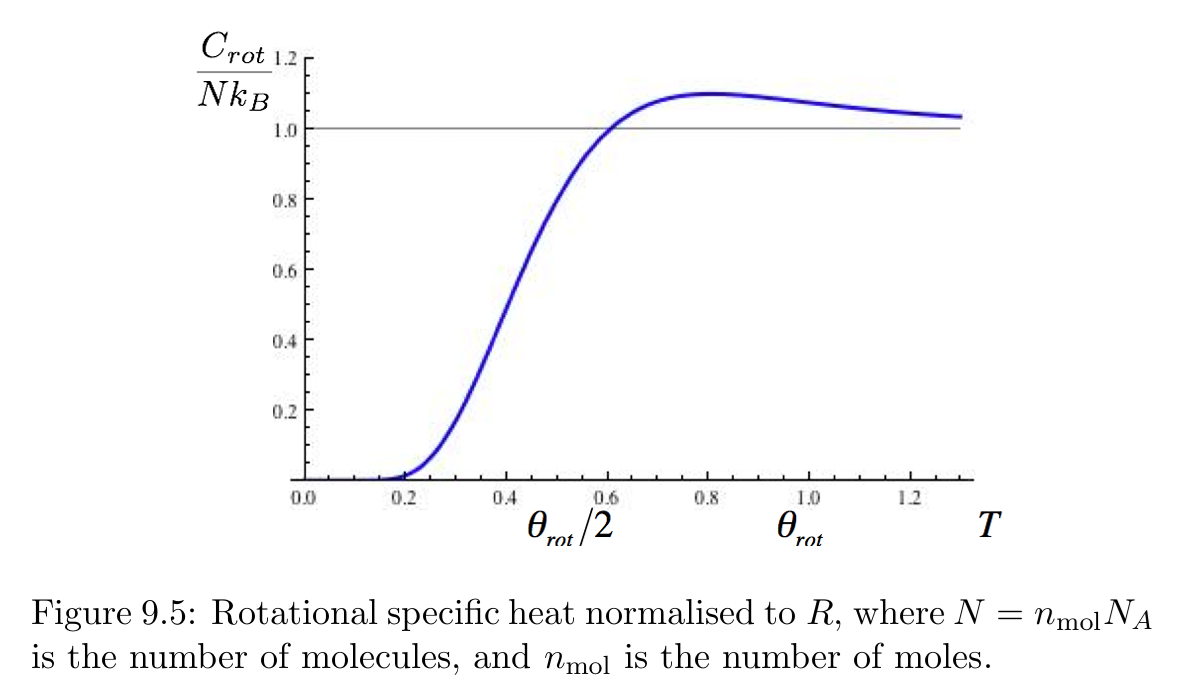
\includegraphics[width=0.6\linewidth]{C_rot vs T.png}
        \item $\lim_{T\rightarrow 0}C_{rot} = 0$
        \item $\lim_{T\rightarrow \infty}C_{rot} = R = N_A k_B$
        \item 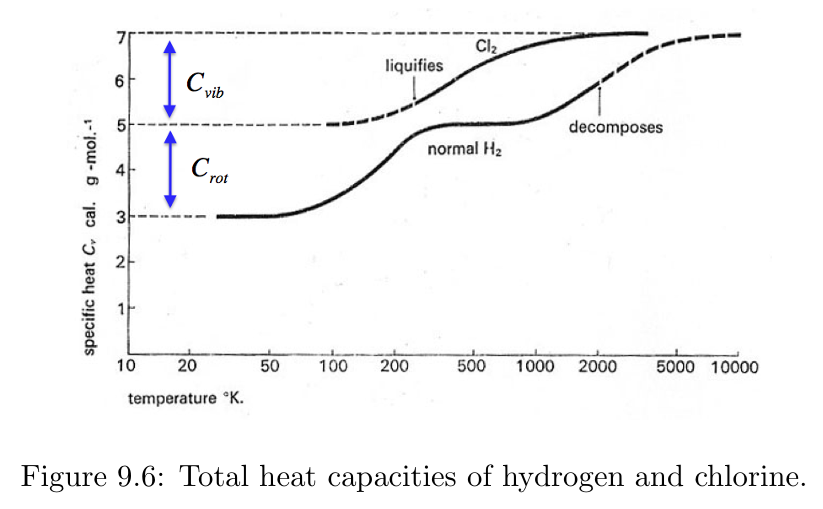
\includegraphics[width=0.6\linewidth]{effect of C_rot, C_vib.png}
        \item Heavier the atom, greater the $I$, smaller the $\theta_{rot}$
        \item unlike $C_{vib}$, $C_{rot}$ has \textbf{lower} characteristic temperature, thus generally present in diatomic gas ($\theta_{rot}<$ freezing point) for elements heavier than $D_2$ (Deuterium)
    \end{itemize}
    \item $\hat{L}^2\psi=l(l+1)\hbar^2\psi$, combining with (\ref{eq:Spherical_Hamiltonian_Simplified})\begin{itemize}
        \item $-\frac{\hbar^2}{2mr^2}\pdv{r}\left(r^2\pdv{R_{n,l}}{r}\right)+\frac{l(l+1)\hbar^2}{2mr^2}R_{n,l}+V(r)R_{n,l}=ER_{n,l}$
        \item substitution $U_{n,l}(r)=rR_{n,l}(r)$, $-\frac{\hbar^2}{2m}\pdv[2]{U_{n,l}}{r}+\left[\frac{l(l+1)\hbar^2}{2mr^2}+V(r)\right]U_{n,l}=EU_{n,l}$
        \item 1D Schr\"odinger, with $V(r)$ replaced by $\frac{\langle\hat{L}^2\rangle}{2mr^2}+V(r)$
        \item Hydrogen-like atom (one electron) \begin{itemize}
            \item $V(r)=-\frac{Ze^2}{4\pi\epsilon_0 r}$
            \item $\boxed{E_n=-\frac{\hbar^2}{2m}\frac{Z^2}{a_0^2}\frac{1}{n^2}}=-\frac{13.6Z^2}{n^2}\mathrm{eV}$,\where{$a_0=\frac{4\pi\epsilon_0\hbar^2}{me^2}=\frac{\hbar}{\alpha mc}=0.53\times 10^{-10}$ is the Bohr radius}
            \item $A=\frac{2m}{\hbar^2}\frac{Ze^2}{4\pi\epsilon_0}$, $\kappa^2=-\frac{2mE_{n}}{\hbar^2}$, $\kappa=\frac{Z}{na_0}$
            \item $R_{n,l}=\frac{U_{n,l}}{r}\propto\sum_{q=0}^{n-(l+1)}c_q r^{q+l}e^{-\kappa r}$
            \item $c_{q+1}=c_q\frac{2\kappa(q+l+1-A/2\kappa)}{(q+1)[q+2(l+1)]}$
            \item \begin{empheq}[box=\fbox]{align*}
                n &\geq 1 \\
                l &= 0,1,2,\cdots,n-1\\
                m_l &= -l,-l+1,\cdots,-1,0,1,\cdots,l-1,l
              \end{empheq}
            \item The energy degeneracy of state $n$ is $\boxed{2\sum_{l=0}^{n-1}(2l+1)=2n^2}$, factor of 2 due to spin
        \end{itemize}
    \end{itemize}
    \item Two body problem $\hat{V} = \hat{V}(|\vb{r}_b-\vb{r}_a|) = \hat{V}(|\vb{r}|)$, then\begin{itemize}
        \item $\hat{H}=\frac{\hat{\vb p}_a^2}{2m_a}+\frac{\hat{\vb p}_b^2}{2m_b}+\hat{V}(\vb{r}_a,\vb{r}_b)$
        \item Centre of mass position $\vb{\hat R}=\frac{m_a\vb{\hat r}_a+m_b\vb{\hat r}_b}{m_a+m_b}$
        \item Relative position $\vb{\hat r}=\vb{\hat r}_b-\vb{\hat r}_a$
        \item \begin{align*}
            \hat{\vb{r}}_a = \frac{m_b}{m_a+m_b}\hat{\vb{r}}+\hat{\vb{R}}\\
            \hat{\vb{r}}_b = -\frac{m_a}{m_a+m_b}\hat{\vb{r}}+\hat{\vb{R}}
        \end{align*}
        \item CoM momentum $\hat{\vb{P}}=i\hbar\pdv{\vb{R}} = i\hbar\left(\pdv{\hat{r}_a}{\hat{R}}\pdv{\hat{r}_a}+\pdv{\hat{r}_b}{\hat{R}}\pdv{\hat{r}_b}\right) = \hat{\vb{p}}_a+\hat{\vb{p}}_b$
        \item relative momentum $\hat{\vb{p}}=i\hbar\pdv{\hat{\vb r}}=\frac{m_a m_b}{m_a+m_b}\left(\frac{\hat{\vb{p}}_a}{m_a}-\frac{\hat{\vb{p}}_a}{m_b}\right)$
        \item $[\hat{\vb R},\hat{\vb p}] = [\hat{\vb r},\hat{\vb P}] = 0$, $[\hat{\vb R},\hat{\vb P}]=[\hat{\vb r},\hat{\vb p}]=i\hbar$
        \item $\dv{\langle\hat{\vb P}\rangle}{t}=\frac{i}{\hbar}\langle \comm{\hat{H}}{\hat{\vb P}}\rangle = 0$
        \item $\hat{H}=\frac{\hat{\vb P}^2}{2m}+\frac{\hat{\vb p}}{2\mu}+\hat{V}(r)$, $\frac{1}{\mu}=\frac{1}{m_a}+\frac{1}{m_b}$
        \item CoM $\hat{H}_{CoM} = -\frac{\hbar^2}{2m}\laplacian_{R}$
        \item Relative $\hat{H}_r = -\frac{\hbar^2}{2m}\laplacian_{r}+V(r)$
        \item $\boxed{\psi(\vb{R},\vb{r})=U(\vb{R})u(\vb{r})}$, $\frac{1}{U(\vb{R})}\hat{H}_{CoM}U(\vb{R})+\frac{1}{u(\vb{r})}\hat{H}_r u(\vb{r})=E\psi(\vb{R},\vb{r})$
        \item $\hat{H}_{CoM}U(\vb{R})=E_{CoM}U(\vb{R})$, $\hat{H}_r u(r)=E_r u(r)$
        \item $\psi(\vb{r}_a,\vb{r}_b)=\boxed{\psi(\vb{R},\vb{r}) = e^{i\vb{P}\cdot\vb{R}/\hbar}\psi_{n,l,m_l}(\vb{r})}$
    \end{itemize}
    \item Spin $\vb{\hat S}=\vb{i}\hat{S}_x+\vb{j}\hat{S}_y+\vb{k}\hat{S}_z$, analogous to $\hat{\vb L}$
    \item \begin{align*}
        \comm{\hat{S}_x}{\hat{S}_y} &= i\hbar\hat{S}_z\\
        \comm{\hat{S}_y}{\hat{S}_z} &= i\hbar\hat{S}_x\\
        \comm{\hat{S}_z}{\hat{S}_x} &= i\hbar\hat{S}_y
    \end{align*}
    \item Because of the commutation relationships, $\comm{\hat{S}^2}{\hat{S}_z} = 0$, $\hat{S}_z\ket{\psi}=m_s\hbar\ket{\psi}$, $\hat{S}^2\ket{\psi}=s(s+1)\hbar^2$
    \item $(2s+1)$ possible values, $m_s=-s,-s+1\cdots,s-1,s$, $s$ is integer or half-integer, $2s+1$ is odd or even
    \item Electron: $2s+1=2$, $s=1/2$, $\langle\hat{S}_z\rangle = \pm\hbar/2$, $\langle\hat{S}\rangle=\sqrt{s(s+1)}\hbar=\frac{\sqrt{3}}{2}\hbar$, $\hat{S}_z\ket{\uparrow}=+\frac{\hbar}{2}\ket{\uparrow}$ is spin up, $\hat{S}_z\ket{\downarrow}=-\frac{\hbar}{2}\ket{\downarrow}$ is spin down
    \item $\boxed{\hat{S}_\pm=\hat{S}_x\pm i\hat{S}_y}$, \begin{itemize}
        \item \begin{empheq}[box=\fbox]{align*}\langle\hat{S}_z\rangle = \pm\hbar/2
            \hat{S}_+\ket{s,m_s}&=\hbar\sqrt{s(s+1)-m_s(m_s+1)}\ket{s,m_s+1}\\
            \hat{S}_-\ket{s,m_s}&=\hbar\sqrt{s(s+1)-m_s(m_s-1)}\ket{s,m_s-1}
        \end{empheq}
        \item Which results in \begin{empheq}[box=\fbox]{align*}
            \hat{S}_+\ket{\uparrow} &= \ket{0}\\
            \hat{S}_+\ket{\downarrow} &= \hbar\ket{\uparrow}\\
            \hat{S}_-\ket{\uparrow} &= \hbar\ket{\downarrow}\\
            \hat{S}_-\ket{\downarrow} &= \ket{0}
        \end{empheq}
        \item $\boxed{\hat{S}_x=\frac{\hat{S}_++\hat{S}_-}{2}, \hat{S}_y=\frac{\hat{S}_+-\hat{S}_-}{2i}$, $\hat{S}_x\ket{\uparrow}=\frac{\hbar}{2}\ket{\downarrow}, \hat{S}_x\ket{\downarrow}=\frac{\hbar}{2}\ket{\uparrow}}$,\begin{empheq}[box=\fbox]{align*}
            \ket{\chi_\pm} &= \frac{1}{\sqrt{2}}(\ket{\uparrow}\pm\ket{\downarrow})\\
            \hat{S}_x\ket{\chi_\pm} &= \frac{\hbar}{2}\ket{\chi_\pm}\\
            \ket{\phi_\pm} &= \frac{1}{\sqrt{2}}(\ket{\uparrow}\pm i\ket{\downarrow})\\
            \hat{S}_y\ket{\phi_\pm} &= \frac{\hbar}{2}\ket{\phi_\pm}\\
        \end{empheq}
    \end{itemize}
    \item $\vb{\hat J} = \vb{\hat L}+\vb{\hat S}$
    \item \begin{align*}
        \comm{\hat{J}_x}{\hat{J}_y} &= i\hbar\hat{J}_z\\
        \comm{\hat{J}_y}{\hat{J}_z} &= i\hbar\hat{J}_x\\
        \comm{\hat{J}_z}{\hat{J}_x} &= i\hbar\hat{J}_y
    \end{align*}
    \item Thus, $\comm{\hat{J}^2}{\hat{J}_z} = 0$, $\hat{J}_z\ket{\psi}=m_j\hbar\ket{\psi}$, $\hat{J}^2\ket{\psi}=j(j+1)\hbar^2\ket{\psi}$, $m_j=-j,\ldots,j$
    \item $\ket{j,m_j} = \sum_{l,m_l,s,m_s}C_{l,m_l,s,m_s}\ket{l,m_l}\ket{s,m_s}$
    \item Total ladder operators $\hat{J}_{\pm}=\hat{L}_{\pm}+\hat{S}_{\pm}$, $\hat{J}_{\pm}\ket{j,m_j}=\hbar\sqrt{j(j+1)-m_j(m_j\pm 1)}\ket{j,m_j\pm 1}$
    \item \begin{tabular}{|c|c|c|c|}
            \hline Spin & 1/2 & 0 & 1\\
            Electron & $\bullet$ & &\\
            Proton & $\bullet$ & &\\
            Neutron & $\bullet$ & &\\
            Quark & $\bullet$ & &\\\hline
            Photon & & &$\bullet$\\
            Phonon & & $\bullet$ &\\
            Higgs boson & & $\bullet$ &\\\hline
        \end{tabular}
    \item Particle exchange operator\begin{itemize}
            \item $\hat{P}_{ij}\ket{\xi_i,\xi_j}=\ket{\xi_j,\xi_i}$
            \item $\langle P\rangle = 1$
            \item $\hat{P}^\dagger_{ij}\hat{P}_{ij}=\hat{I} = \hat{P}_{ij}^2$
            \item $\dv{\langle P\rangle}{t}=\frac{i}{\hbar}\langle[\hat{H},\hat{P}]\rangle = 0$
            \item $[\hat{A},\hat{P}_{ij}]=0$, $\hat{P}_{ij}$ compatible with all observables
        \end{itemize}
    \item The \emph{symmetrisation postulate}: states of $N$ identical particles are either exchange symmetric or exchanged antisymmetric
    \item The \emph{spin statistics theorem}: integer spin particles are bosons $p_B(\epsilon)=\frac{1}{\exp[(\epsilon-\mu)/k_B T]-1}$, half-dd-integer spin particles are fermions $p_F(\epsilon)=\frac{1}{\exp[(\epsilon-\mu)/k_B T]+1}$
    \item Two particle basis $\ket{\alpha}\ket{\alpha}$, $\ket{\alpha}\ket{\beta}$, $\ket{\beta}\ket{\alpha}$, $\ket{\beta}\ket{\beta}$ can be expressed as $\ket{\alpha}\ket{\alpha}$, $\ket{s}=\frac{1}{\sqrt{2}}[\ket{\alpha}\ket{\beta}+\ket{\beta}\ket{\alpha}]$,
     $\ket{a}=\frac{1}{\sqrt{2}}[\ket{\alpha}\ket{\beta}-\ket{\beta}\ket{\alpha}]$, $\ket{\beta}\ket{\beta}$.
     $\ket{a}$ is antisymmetric ($\hat{P}_{\alpha\beta}\ket{a}=-\ket{a}$), the others are symmetric ($\hat{P}_{\alpha\beta}\ket{s}=\ket{s}$)
    \item $N$ bosons placed in $n$ states, each having $m_n$ bosons\begin{itemize}
            \item $\ket{1,2,1}$, $\ket{1,1,2}$ and $\ket{2,1,1}$ are the same state, to use previous notations, we add them up and normalize
            \item The state is described by $\frac{2!1!}{3!}\left[\ket{1,1,2}+\ket{1,2,1}+\ket{2,1,1}\right]$
            \item generally this symmetric/boson state is \newline
                $\ket{a\ldots r\ldots z}^s=\sqrt{\frac{\prod_n(m_n!)}{N!}}\sum_P\ket{\xi^a}\cdots\ket{\xi^r}\cdots\ket{\xi^z}$
                \where{$P$ loops through all permutations}
        \end{itemize}
    \item $N$ fermions\begin{itemize}
        \item for fermions, each occupy a unique state ($m_n=1$ only)
        \item $\ket{1,1,2}$ does not exist; cannot have two fermions being 1
        \item $\ket{123}^a = \ket{1,2,3}+\ket{2,3,1}+\ket{3,1,2}-\ket{1,3,2}-\ket{3,2,1}-\ket{2,1,3}$
        \item $\ket{a\ldots r\ldots z}^a=\frac{1}{\sqrt{N!}}\sum_P(-1)^{f(P)}\ket{\xi^a}\cdots\ket{\xi^r}\cdots\ket{\xi^z} = \frac{1}{\sqrt{N!}}\begin{vmatrix}
                    \ket{\xi^1} & \ket{\xi^1} & \cdots & \ket{\xi^1}\\
                    \ket{\xi^2} & \ket{\xi^2} & \cdots & \ket{\xi^2}\\
                    \vdots & \vdots & \ddots & \vdots\\
                    \ket{\xi^N} & \ket{\xi^N} & \cdots & \ket{\xi^N}\\
                \end{vmatrix}$
                \where{$f(P)$ is the number of swaps needed to get permutation $P$ from original order,\newline
                            the determinant is the \emph{Slater determinant}}
    \end{itemize}
    \item Davisson \& Germer, electrons have de Broglie wavelength (they diffract off a lattice with Bragg reflection, $d\sin\theta=n\lambda$)        
    \item Bohr's atom, discrete angular momentum makes electrons stay in stable orbit
    \item Planck's blackbody, discrete photon energy/cavity mode produces correct equation, solved the ultaviolet catastrophe in Rayleight-Jeans law
    \item Photoelectric effect, work function, intensity useless frequency important
    \item Stern-Gerlach (2 splits, not odd number of 2l+1 splits, due to spin)\\
        \includegraphics*[width=0.4\linewidth]{stern_gerlach.png}
\end{enumerate}

\end{document}